\documentclass[
fontsize=11pt,
paper=a4,
numbers=noenddot,
parskip=half,
div=13
]{scrartcl}

\usepackage[bottom=3cm, top=3cm]{geometry}

\usepackage[utf8]{inputenc}
\usepackage[T1]{fontenc}

\usepackage[backend=biber]{biblatex}
\addbibresource{bibliography.bib}

\newcommand{\HRule}{\rule{.9\linewidth}{.6pt}}

\usepackage[light]{kpfonts}
\usepackage[activate={true,nocompatibility},final,tracking=true,kerning=true,spacing=true,factor=1100,stretch=10,shrink=10]{microtype}
\recalctypearea

%------------------------------------------------------
%	LAYOUT
% -----------------------------------------------------
\usepackage[hidelinks]{hyperref}  
\hypersetup{pdftitle={Software Practical -- Uncertainty Quantification}}
\hypersetup{pdfauthor={Nils Friess}}
\hypersetup{colorlinks=false}

\usepackage{setspace}
\onehalfspacing

% MATH PACKAGES
\usepackage{mathtools}
\usepackage{amsthm}
\usepackage{amssymb}
\usepackage{bm}
\usepackage{showlabels}

% OTHER PACKAGES
\usepackage{todonotes}
\usepackage[ruled,vlined,resetcount]{algorithm2e}
\SetKwInput{KwData}{Input}

\usepackage{enumitem}

\usepackage[cache=false]{minted}

% NEW DEFINITIONS AND OTHER SETUP

\addtokomafont{disposition}{\rmfamily}

%------------------------------------------------------
%	ABBREVIATIONS
% -----------------------------------------------------
\newcommand{\ie}{i.\,e.\ }
\newcommand{\eg}{e.\,g.\ }
\newcommand{\wrt}{w.\,r.\,t.\ }

%%% Local Variables:
%%% TeX-command-extra-options: "-shell-escape"
%%% mode: latex
%%% TeX-master: "main"
%%% End:


\def\R{\mathbb{R}} 
\def\N{\mathbb{N}}
\def\Z{\mathbb{Z}}
\def\K{\mathbb{K}}
\def\C{\mathbb{C}}
\def\Rp{\mathbb{R}_{+}}
\def\F{\mathbb{F}}
\def\I{\mathbb{I}}

\def\iff{~\Leftrightarrow~}

\def\eps{\mathtt{eps}}
% function spaces
\def\CC{\mathscr{C}}
% space of polynomials
\def\P{{\mathcal{P}}}

% integrals, derivatives
\def\d{\mathrm{d}}
\def\dx{\,\mathrm{d}x}
\def\dt{\,\mathrm{d}t} 

\def\rd{\text{rd}}

\def\Df{\mathrm{D}f}

\def\O{\mathcal{O}}

\def\rq{\mathrm{R}}

% duality pairing
\def\<{\langle}
\def\>{\rangle}

% Swap the definition of \abs* and \norm*, so that \abs
% and \norm resizes the size of the brackets, and the 
% starred version does not.
\DeclarePairedDelimiter\abs{\lvert}{\rvert}%
\DeclarePairedDelimiter\norm{\lVert}{\rVert}%

\makeatletter
\let\oldabs\abs%
\def\abs{\@ifstar{\oldabs}{\oldabs*}}
%
\let\oldnorm\norm%
\def\norm{\@ifstar{\oldnorm}{\oldnorm*}}
\makeatother

\makeatletter
\newcommand*{\tp}{%
  {\mathpalette\@transpose{}}%
}
\newcommand*{\@transpose}[2]{%
  % #1: math style
  % #2: unused
  \raisebox{\depth}{$\m@th#1\intercal$}%
}
\makeatother

\makeatletter
\newcommand*{\herm}{%
  {\mathpalette\@hermitian{}}%
}
\newcommand*{\@hermitian}[2]{%
  % #1: math style
  % #2: unused
  \raisebox{\depth}{$\m@th#1{\mathrm{H}}$}%
}
\makeatother

% vertical equals 
\newcommand{\verteq}{\rotatebox{90}{$\,=$}}
% underset with vertical equals
\newcommand{\equalto}[2]{\underset{\scriptstyle\overset{\mkern4mu\verteq}{#2}}{#1}}

% for fractions with bigger elements or nested fractions
\newcommand{\ffrac}[2]{\ensuremath{\frac{\displaystyle #1}{\displaystyle #2}}}

\DeclareMathOperator{\rang}{rang}
\DeclareMathOperator{\cond}{cond}
\DeclareMathOperator{\diag}{diag}
\DeclareMathOperator{\im}{im}
\DeclareMathOperator{\spr}{spr}

\DeclareMathOperator*{\argmax}{arg\,max}
\DeclareMathOperator*{\argmin}{arg\,min}

\DeclarePairedDelimiterX{\inp}[2]{\langle}{\rangle}{#1, #2}

\newcommand*{\mat}[1]{\bm{#1}}
\let\oldvec=\vec
\renewcommand{\vec}[1]{\mathbf{#1}}

%%%%%%%%%%%%%%%%%%%%%%%%%%%%%%%%%%%%%%%%%%%%%%%%
%%%%% Theorem environments %%%%%%%%%%%%%%%%%%%%%
\newtheorem{theorem}[algocf]{Theorem}
\newtheorem{corollary}[algocf]{Corollary}
\newtheorem{lemma}[algocf]{Lemma}
\newtheorem{proposition}[algocf]{Proposition}

\theoremstyle{definition}
\newtheorem{definition}[algocf]{Definition}
\newtheorem{example}[algocf]{Example}
\newtheorem*{remark*}{Remark}
\newtheorem{remark}[algocf]{Remark} 
 
%%% Local Variables:
%%% mode: latex
%%% TeX-master: "main"
%%% End:
 

% DRAFT PACKAGES
%\usepackage{showlabels}

\title{{\normalsize Software Practical Uncertainty Quantification}\\Report}

\begin{document} 
\title{ \normalsize
  \HRule\\[0.5cm]
  \large \textsc{Software practical --- Uncertainty Quantification}\\
  \LARGE {Implementation of a C++ Particle Filter Library}\\
  \HRule\\[0.5cm]
  \normalsize Winter semester 2019 \vfill }

\date{}

\author{ \large
  Submitted by: \textbf{Nils Friess}\\
  {\small\today}\\[3ex]
  \normalsize
  Supervisors: Prof.\ Robert Scheichl, Gianluca Detommaso \\
  \normalsize Heidelberg University }

\clearpage\maketitle
\thispagestyle{empty}
\newpage
\setcounter{page}{1}

\section*{Introduction}\label{sec:intro}
In this report we present an implementation of a Particle Filter in
C++. Before discussing the actual implementation we give the
theoretical details of the method in this section. We start by giving
a brief overview of the method before discussing the individual steps
in more detail.

We remark here, that the naming in these methods is highly ambiguous
and varies greatly from author to author and even in different
publications of the same authors. We use -- with some exceptions --
the naming and notation used in~\cite{doucet} and highlight parts
where the naming differs from other publications.

\subsection*{Overview of a Particle Filter}
A Particle Filter is a Sequential Monte Carlo (SMC)
method\footnote{Some authors use the terms \emph{Particle Filter} and
  \emph{SMC method} synonymously. Doucet and Johansen develop
  in~\cite{doucet} a framework in which Particle Filters are only one
  specific method in the much broader class of SMC methods. They argue
  that this distinction allows for a better understanding of these
  methods. In this report, we are only interested in the
  \emph{filtering problem} and we will introduce it without discussing
  the more general notion of SMC methods as given by Doucet and
  Johansen.} that is used to estimate the state of a system that
changes over time using only noisy and/ or partial observations of the
system's state. This will be done in a Bayesian framework where one
attempts to construct the posterior probability density function (pdf)
of the state based on the observations. We make the following
assumptions:
\begin{enumerate}[label=(A\arabic*)]
\item The model describing the initial state and the evolution of the
  internal state in time is available in a probablistic form.
\item The model that relates the observations to the internal state is
  available in a probabilistic form.
\item The observations are only available sequentially, not as a batch
  (ie. we assume that we receive new measurments sequentially in
  time).
\end{enumerate}
Due to (A3) we aim at a recursive method that does neither require to
store nor to reprocess all the previous information when a new
observation becomes available. To formalise the first two assumptions
we will use the notion of \emph{hidden markov models}.

Such models consist of the triplet
\begin{align*}
  \label{eq:hmm:1}
  X_0 &\sim \mu(x_0)\,,\\
  X_n \mid (X_{n-1} = x_{n-1}) &\sim p(x_n \mid x_{n-1})\,,\\
  Y_n \mid (X_n = x_n) &c\sim p(y_n \mid x_n) \,,
\end{align*}
where
\begin{itemize}
\item $n \in \N$ denotes discrete time;
\item $X_n$ is the $d_x$-dimensional state of the system taking values
  in $\R^{d_x}$;
\item $p(x_0)$ is the prior probability density fumction (pdf) of the
  system's state;\footnote{ With abuse of notation we denote by $p(x)$
    the pdf of the random variable $X$. For two random variables $X$
    and $Y$ the corresponding (possibly different) density functions
    are denoted by $p(x)$ and $p(y)$ respectively; $p(x,y)$ denotes
    the joint pdf and $p(x \mid y)$ is the conditional pdf of $X$
    given $Y = y$.}
\item $Y_n$ is the $d_y$-dimensional vector of observations which is
  assumed to be conditionally iindependent of all other observations
  given the state $X_n$,
\item $p(y_n \mid x_n)$ is the conditional pdf of $Y_n$ given
  $X_n = x_n$.
\end{itemize}
Assumptions (A1) and (A2) then state that all these pdfs are known.
Our goal is now to estimate the distribution $p(x_n \mid y_{1:n})$,
where $y_{1:n} \coloneqq (y_1, y_2, \dotsc, y_n)$. This is often
referred to as the \emph{filtering problem} or
\emph{tracking}.\footnote{Note that Docuet and Johansen \emph{do not}
  call this the filtering problem~\cite{doucet}. They reserve this
  term for the estimation of the joint distributions
  $p(x_{1:n} \mid y_{1:n} )$. Since we are only concerned with
  estimating the marginal distribution $p(x_n \mid y_{1:n} )$ we will
  still refer to this problem as filtering.}

% In principle, this is could be done in two steps: prediction and
% update. By the Chapman-Kolmogorov equation we first obtain
% \begin{align*}
%   p(x_{k+1} \mid y_{1:k}) &= \int p(x_{k+1} \mid x_k, y_{1:k}) p(x_k \mid y_{1:k}) \dx_k \\
%                           &= \int f(x_{k+1} \mid x_k) p(x_k \mid y_{1:k}) \dx_k \,,
% \end{align*}
% where we used the Markov property of the system, \ie
% \[
%   p(x_{k+1} \mid x_k, y_{1:k}) = p(x_{k+1} \mid x_k) = f(x_{k+1}
%   \mid x_k) \,.
% \]
% Once a new observation $y_{k+1}$ becomes available we can update our
% beliefs about the system's state using Bayes' theorem
% \[
%   p(x_{k+1} \mid y_{1:k+1}) = \frac{ p(y_{k+1} \mid x_{k+1})
%   p(x_{k+1} \mid y_{1:k}) }{ p(y_{k+1} \mid y_{1:k}) }\,,
% \]
% where the normalising constant
% \begin{align*}
%   p(y_{k+1} \mid y_{1:k}) &= \int p(y_{k+1} \mid x_{k+1}) p(x_{k+1} \mid y_{1:k}) \dx_{k+1} \\
%                           &= \int g(y_{k+1} \mid x_{k+1}) p(x_{k+1} \mid y_{1:k}) \dx_{k+1}
% \end{align*}
% depends on the likelihood function defined by the model
% in~\eqref{eq:hmm:2}. Putting these two steps together, we obtain a
% recursive formula using the previous filtered state of the system
% $p(x_{k} \mid y_{1:k})$ and a new observation $y_{k+1}$ to compute
% the current state of the system.
\todo{1-step-predictor (Chapman-Kolmogorov)}
In a restrictive set of cases this distribution can be computed
exactly (\eg when $p(y_t \mid y_t)$ is linear and the posterior of the
system is Gaussian~\cite[175]{arulampalam} or when the underlying
state space of the Markov model is finite, cf.~\cite[Example
1]{doucet}). In a more general nonlinear non-Gaussian setting,
approximative methods such as particle filters are
necessary. Therefore, in practice a different approach is used.

\section*{(Sequential) importance sampling}
The central idea of Particle filters is to represent the posterior of
the system $p(x_k \mid y_{1:k})$ at some time $k$ as a weighted set of
samples, so called \texttt{particles}, denoted by
$\{ x^{(i)}_k, w^{(i)}_k \}.$ If we ignore for a moment the weights
and assume that the samples are from the desired distribution, \ie
\[
  x^{(i)}_k \sim p(x_k^{(i)} \mid y_{1:k}), \quad i = 1, \dotsc, N
\]
the Monte carlo method approximates $p(x_k \mid y_{1:k})$ by the
empirical measure\footnote{Again, we slightly abuse the notation for
  simplicity; the alternations required for a rigorous
  measure-theoretic formulation are straightforward.}
\begin{equation}
  \label{eq:empirical_measure}
  \hat{p}(x_k \mid y_{1:k}) = \frac{1}{N} \sum_{i = 1}^N
  \delta_{x_k^{(i)}}(x_k)\,,
\end{equation}
where $\delta_x(\cdot)$ denotes the Dirac delta centered at $x$. The
expectation of a test function $f : \R^{d_x} \rightarrow \R$ given by
\[
  \mathbb{E}[f(x_k) \mid y_{1:k}] = \int f(x_k) p(x_k \mid y_{1_k})
  \dx_k
\]
is then estimated by
\[
  {\mathbb{E}}^{\text{MC}}[f(x_k) \mid y_{1:k}] = \int f(x_k)
  \hat{p}(x_k \mid y_{1_k}) \dx_k = \frac{1}{N} \sum_{i=1}^N
  f(x^{(i)}_k)\,.
\]
It is well-known that the variance of the approximation error using
this estimator decreases \emph{independent of $d_x$} with a rate of
$\mathcal{O}(N^{-1})$. However, often it is either impossible or
practically intractable to sample from the posterior directly and
thus, in practice one often relies on a technique called
\emph{importance sampling}.

We start by choosing an \emph{importance density}
$q(x_k \mid y_{1:k})$ and draw $N$ samples $x^{(i)}_k$ from it. If we
would use these samples to approximate $p(x_k \mid y_{1:k})$ as
in~\eqref{eq:empirical_measure} the result would obviously not be
accurate in general. To correct this bias we introduce
\emph{importance weights}
\begin{equation}
  \label{eq:importance_weights}
  w_k^{(i)} \propto \frac{p(x_k^{(i)} \mid y_{1:k})}{q(x_k^{(i)} \mid
    y_{1:k})} \,,
\end{equation}
that we require to be normalised such that $\sum_i w_k^{(i)} = 1$. We
can now approximate the target density by
\begin{equation}
  \label{eq:karget:approx}
  p(x_k \mid y_{1:k}) \approx \sum_{i=1}^N w_k^{(i)} \delta_{x_k^{(i)}}(x_k) \,.
\end{equation}
This technique is called \emph{importance sampling}. Expectations of
test functions can then be estimated by
\[
  \mathbb{E}^{\text{MC}}[f(x_k) \mid y_{1:k}] = \sum_{i=1}^N
  w_k^{(i)}f(x_k^{(i)}) \,.
\]
Due to assumption (A3) ideally we would like a recursive formula to
update the weights a each step. To obtain such a formula we consider
the full posterior $p(x_{0:k} \mid y_{1_k})$ and express it in terms
of the posterior at the previous time step and the known pdf's
$p(y_k \mid x_k)$ and $p(x_k \mid x_{k-1})$:
\begin{align*}
  p(x_{0:k} \mid y_{1:k}) &\propto p(y_k \mid x_{0:k}, y_{1:k-1}) p(x_{0:k} \mid y_{1:k-1}) \\
                          &= p(y_k \mid x_k) p(x_k \mid x_{0:k-1}, y_{1:k-1}) p(x_{0:k-1} \mid y_{1:k-1}) \\
                          &= p(y_k \mid x_k) p(x_k \mid x_{k-1}) p(x_{0:k-1} \mid y_{1:k-1})\,,
\end{align*}
where we used Bayes' theorem and the properties of the system
described earlier. If in addition we choose an importance density that
factorizes such that
\[
  q(x_{0:k} \mid y_{1:k}) = q(x_k \mid x_{0:k-1}, y_{1:k}) q(x_{0:k-1}
  \mid y_{1:k-1})
\]
the weights~\eqref{eq:importance_weights} can be written as
\begin{align*}
  w_k^{(i)} &\propto \frac{p(y_k \mid x_k^{(i)}) p(x_k^{(i)} \mid x_{k-1}^{(i)}) p(x_{0:k-1}^{(i)} \mid y_{1:k-1})}{q(x_k^{(i)} \mid x_{0:k-1}^{(i)}, y_{1:k}) q(x_{0:k-1}^{(i)} \mid y_{1:k-1})} \\
            &= \frac{p(y_k \mid x_k^{(i)}) p(x_k^{(i)} \mid x_{k-1}^{(i)})}{q(x_k^{(i)} \mid x_{0:k-1}^{(i)}, y_{1:k})} w^{(i-1)}_k \,.
\end{align*}
Since in our case, we are only interested in estimating the filtered
posterior $p(x_k \mid y_{1:k})$ we choose an importance density
$q(x_k \mid x_{0:k-1}, y_{1:k}) = q(x_k \mid x_{k-1}, y_{k})$ that
only depends on $x_{k-1}$ and $y_k$. Then, merely $x_k^{(i)}$ is held
in memory and the path $x_{0:k-1}^{(i)}$ and history of observations
$y_{1:k-1}$ need not be stored. The weights can the recursively be
computed by
\begin{equation}
  \label{eq:weight_update}
  w_k^{(i)} \propto \frac{p(y_k \mid x_k^{(i)}) p(x_k^{(i)} \mid
    x_{k-1}^{(i)})}{q(x_k^{(i)} \mid x_{k-1}^{(i)}, y_{1:k})}
  w^{(i-1)}_k \,.
\end{equation}
This is usually referred to as \emph{sequential} importance sampling.
We summarise the results up to this point in Algorithm~\ref{alg:sis}.
Note, that since at time $k = 0$ no observation or previous state is
available, we sample from the (known) prior and weigh all particles
equally.
\begin{algorithm}[t]
  \SetAlgoLined \KwData{$n$ observations $y_1, y_2, \dotsc, y_n$;\quad
    number of particles $N$} Sample $x_0^{(i)} \sim \mu(x_0^{(i)})$ \;
  Set weights $w_0^{(i)} = 1/N$\;
  \For{$k = 1,2, \dotsc, n$}{ Sample
    $x_k^{(i)} \sim q(x_k^{(i)} \mid x_{k-1}^{(i)}, y_k)$. \; Compute
    weights according to~\eqref{eq:weight_update}. \; Normalise
    $w_k^{(i)} = \tilde{w}_k^{(i)} / \sum_j \tilde{w}_k^{(j)}$ }
  \caption{Sequential importance sampling}\label{alg:sis}
\end{algorithm}

Using this approach alone, however, leads to \emph{degeneracy} of the
particles. It can be shown that the variance of the weights can only
increase at every step, which implies that the algorithm will
eventually produce a single non-zero weight $w^{(i)} \approx 1$,
carrying all the statistical information with the rest of the weights
converging to zero. This is visualised in Figure~\ref{fig:weights}
where we plotted a histogram of the weights after the first few time
steps. One can clearly see that after a few steps almost all the
weights are zero. To account for this problem, we introduce another
technique called \emph{resampling}.
\begin{figure}[hbtp]
  \centering \makebox[\textwidth][c]{%
    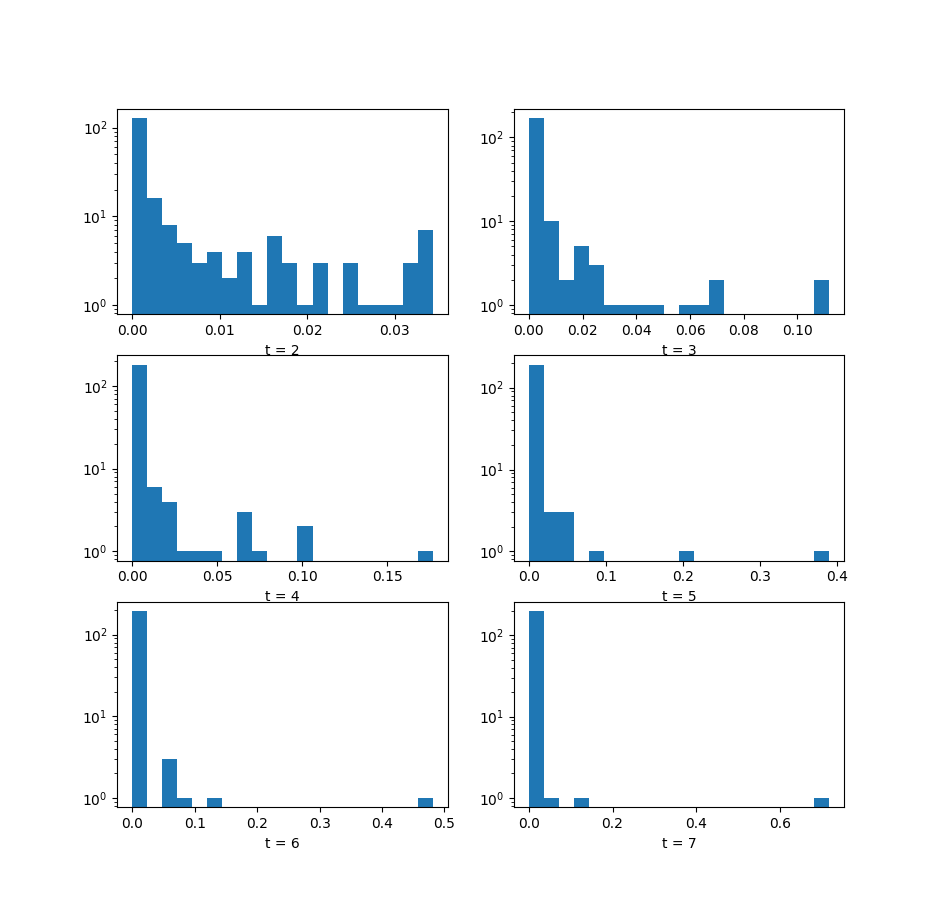
\includegraphics[width=1.3\textwidth]{figures/Figure_weights.png}
  }
  \caption{A histogram of 200 weights after just a few
    iterations. Almost all the weights are zero at $k = 7$ which
    demonstrates the degeneracy of the particles.}
  \label{fig:weights}
\end{figure}

\section*{Resampling}
We are going to present two resampling strategies in this section. The
overall goal of all resampling methods is to remove particles with
negligible weights with a high probability and replicate those with
high weights. After resampling, the future particles are more
concentrated in domains of higher posterior probability, which entails
improved estimates. It can, of course, happen that a particle with a
low weight at time $t$ has a high weight at time $t+1$, in which case
resampling could be wasteful. It should also be mentioned that if
particles have (unnormalised) weights with a small variance,
resampling might be unnecessary. This is discussed briefly at the end
of this section. As above, we denote by
$\{ x^{(i)}, w^{(i)} \}_{1 \le i \le N}$ the set of particles with
their associated weights at some time $k$ (which is omitted in the
notation). We assume that the weights have already been normalised,
i.\,e.\ $\sum_i w^{(i)} = 1$. We further denote by
$\{ \tilde{x}^{(i)}, \tilde{w}^{(i)} \}_{1 \le i \le N}$ the particles
and weights after resampling took place. We require the particles
$\tilde{x}^{(i)}$ to be weighted equally which implies, since we also
require the weights to be normalised, that $\tilde{w}^{(i)} = 1/N$.

The use of resampling to improve importance sampling was originally
introduced by Gordon et al, see~\cite{gordon}, laying the ground for
Particle filters and SMC methods in general. The resampling methods
presented here are two of the most popular amongst the literature,
see~\cite{douc}.  The most simple resampling strategy, called
\emph{multinomial resampling} is not discussed here due to its poor
performance compared to other techniques. It only is mentioned because
it is the method introduced by Gordon et al. in~\cite{gordon} as part
of the\emph{ bootstrap filter}, that uses the prior as the proposal
density (c.\,f.\ Example~\ref{ex:lv1}).

Both the methods presented in the following are based on drawing
samples from the point mass distribution
$\sum_{j=1}^N w^{(j)} \delta_{X^{(j)}}$. In practice, this is achieved
by repeated uses of the inversion method, which itself uses the
empirical cumulative distribution function (cdf) associated with the
weights. This is based on the following fact:

\textbf{Claim.}\quad If $U$ is a uniform random variable on $(0,1]$
then $X = F^{-1}(U)$ has distribution $F$, where $F$ is the cumulative
distribution function of $X$ and
$F^{-1}(t) = \min \{ x \mid F(x) = t \}$ is the inverse cdf.

\textbf{Proof.}\quad Let $U \sim \mathcal{U} (0,1]$. Then
\begin{align*}
  P(F^{-1}(U) \le x) &= P(\min \{x \mid F(x) = U \} \le x ) && \text{(definition of $F^{-1}$)} \\
                     &= P(U \le F(x)) \\
                     &= F(x) && \text{(definition of distribution of $U$)}\,.
\end{align*}
\hfill$\square$

The inversion method can be explained visually as follows. We plot the
empirical cdf of the weights and sample from
$U \sim \mathcal{U}(0,1]$. We denote the actual value of the sample by
$u$. We then draw a horizontal line from the coordinate $(0,u)$ to the
right until it intersects one of the bars, see
Figure~\ref{fig:ecdf}. The index of the bar that is intersected
determines the new sample.

\begin{figure}[htpb]
  \centering 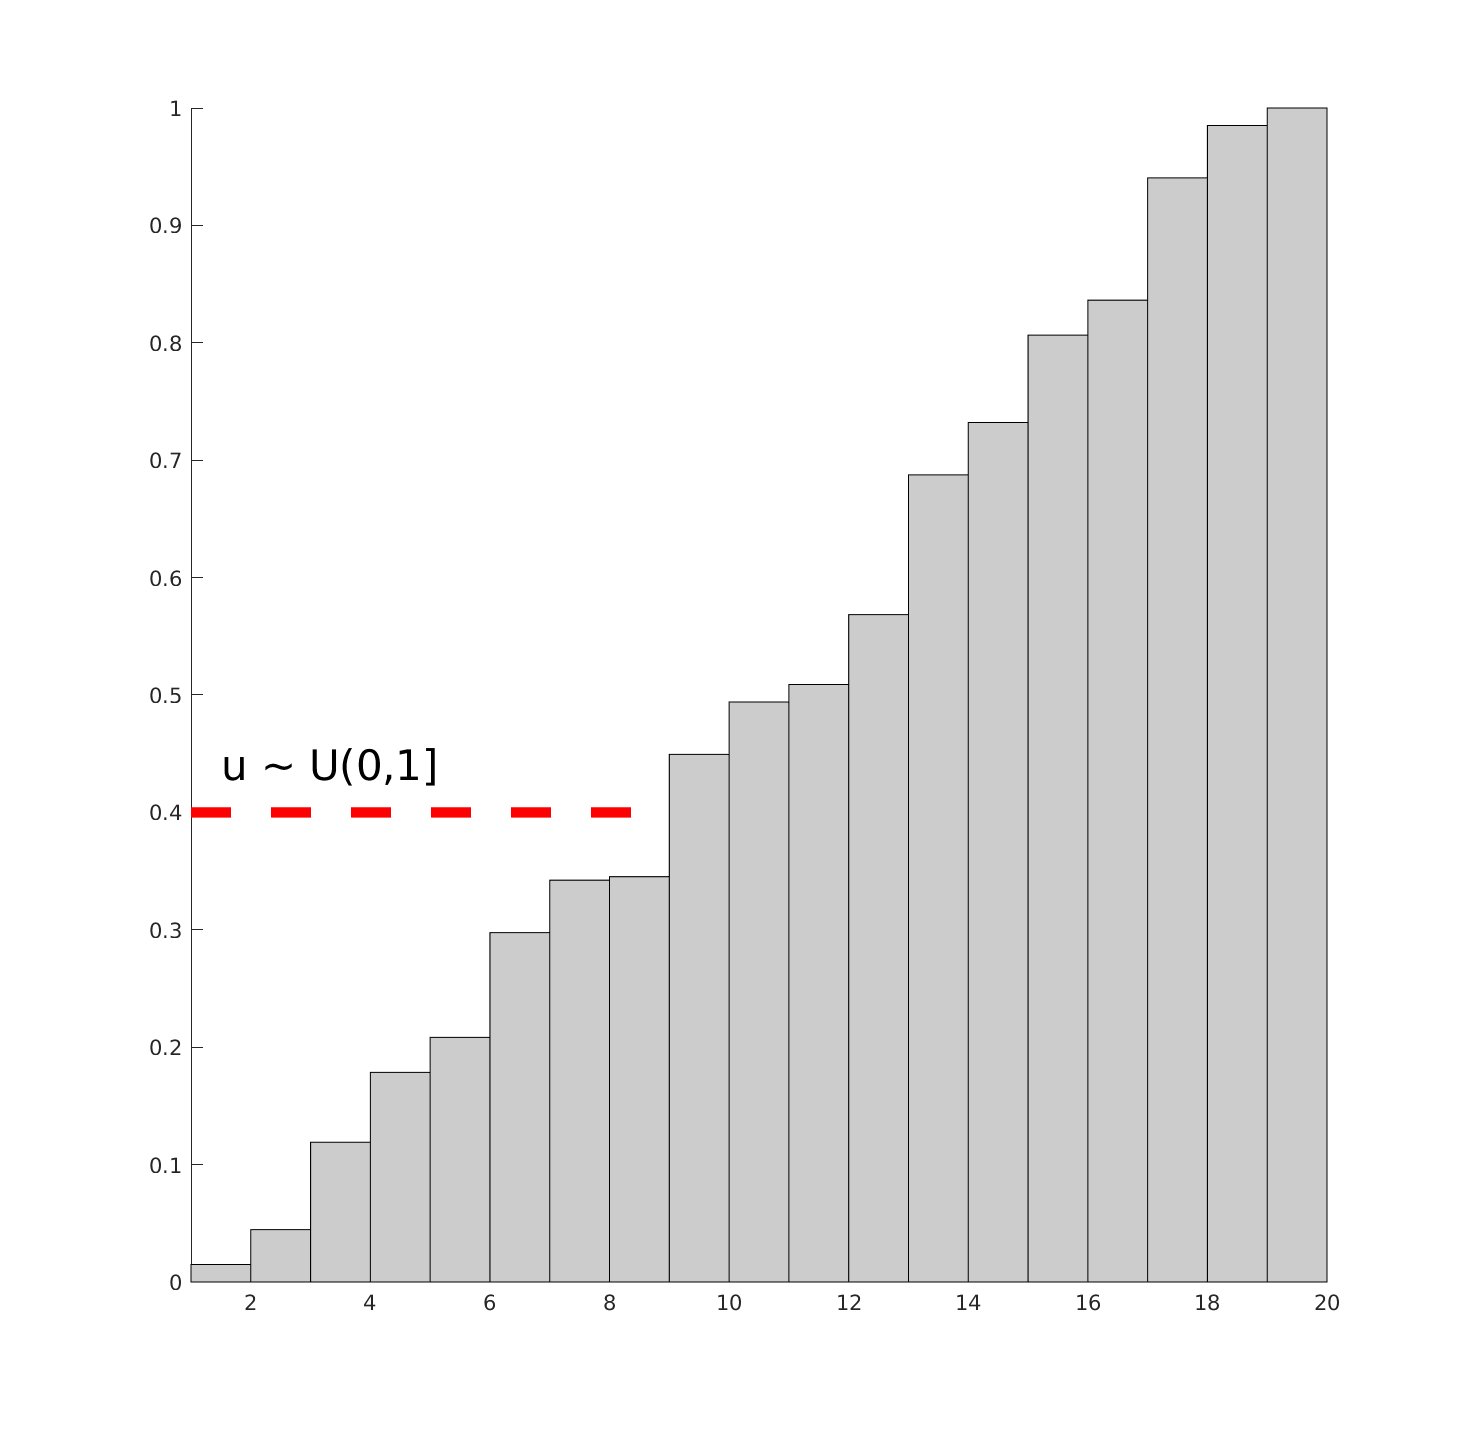
\includegraphics[width=\textwidth]{figures/ecdf.png}
  \caption{Visualisation of the inversion method. The bars represent
    the empirical cumulative distribution function associated with a
    set of 19 weights. The red line is horizontally drawn from the
    value of $u$ at the vertical axis until it ``hits'' a bar. The
    index of the bar yields the generated sample (in this case the new
    sample is therefore 9). }
  \label{fig:ecdf}
\end{figure}

In our case, we do not draw just one sample $U$ but we generate $N$
different samples $\{U_i\}_{1 \le i \le N}$ in such a way that they
are sorted in ascending order. For every of these samples (from lowest
to highest) we look for the intersected bar and add its index to a
list. This list then corresponds to the indices of the particles that
should be resampled. Consider the following example: Suppose we had
five particles and the list of indices after the resampling reads
$\{1,3,4,4,5\}$. Then, particles $X^{(1)},X^{(3)},X^{(5)}$ should be
resampled, particle $X^{(4)}$ should even be duplicated. Particle
$X^{(2)}$, however, will be dropped. In other words, the particles
after the resampling are
\begin{gather*}
  \tilde{X}^{(1)}=X^{(1)},\ \tilde{X}^{(2)}=X^{(3)},\ \tilde{X}^{(3)}=X^{(4)},\\
  \tilde{X}^{(4)}=X^{(4)},\ \tilde{X}^{(5)}=X^{(5)}\,.
\end{gather*}

The two strategies presented in the following only differ in the way
the $U_i$s are generated. We summarise the results in
Algorithm~\ref{alg:resampling}.

\begin{algorithm}[htpb]
  \SetAlgoLined \KwData{$N$ samples $U_i \sim \mathcal{U}(0, 1]$
    sorted in ascending order;\ list of weights} \KwResult{List of
    indices $I$ that represent that particles to be resampled} $C$ =
  \texttt{cumsum}(weights) \tcp*{Generate the empirical cdf as list of
    cumulated sums} $I$ = zeros(N)\; $i,j = 0$\; \While{$i < N$}{
    \eIf(\tcp*[h]{Found intersecting bar}){$U_i < C_j$}{ $I_i = j$\;
      $i = i+1$\; } { $j = j + 1$\; } }
  \caption{Resampling using the empirical cdf}\label{alg:resampling}
\end{algorithm}

Here, the function \texttt{cumsum} is assumed to work in the same way
as, for example, MATLAB's or NumPy's \texttt{cumsum} function. That
is, \texttt{cumsum([1,2,3,4])} should return \texttt{[1,3,6,10]}.

\subsection*{Systematic Resampling}
This algorithm separates the sample space into $N$ divisions. One
random offset, drawn from a $\mathcal{U}[0, 1)$ distribution, is used
to choose where to sample from for all divisions. This guarantees that
every sample is exactly $1/N$ apart.

In other words, the $U_i$s are generated by sampling
$\tilde{U} \sim \mathcal{U}[0, 1)$ and defining
\[
  U_i = \frac{\tilde{U} + i-1}{N} \quad \text{for } i = 1, \dotsc, N
  \,.
\]

\subsection*{Stratified Resampling}
This algorithm is similar to the previous one, its aim is to make
selections relatively uniformly across the particles. We start by
partitioning the $(0,1]$ interval into $N$ disjoint sets,
$(0,1] = (0, 1/N] \cup (1/N, 2/N] \cup \dotsm \cup ((N-1)/N, 1]$. The
$U_i$s are then drawn independently in each of the sub-intervals:
\[
  U_i \sim \mathcal{U}((i-1)/N, i/N]\,.
\]

We mentioned earlier that resampling might be unnecessary if the
weights are sufficiently uniform and we would like to have a criterion
allowing us to check whether resampling should be performed. To that
end the effective sampling size ($ESS$) is often used which can be
estimated using
\[
  ESS \approx {\left( \sum_{i=1}^N {\left( w_t^{(i)} \right)}^2
    \right)}^{-1} \,,
\]
where the weights $w_t^{(i)}$ are assumed to be already normalised
(for more details, see~\cite[179]{arulampalam}). If the variance of
the weights is maximal, i.\,e.\ if all but one of the weights are
zero, the value of $ESS$ is 1. If, however, the weights all have the
same value $w_t^{(i)} = 1/N$ the value of $ESS$ is $N$, since
\[
  {\left( \sum_{i=1}^N {\left( \frac{1}{N} \right)}^2 \right)}^{-1} =
  {\left( N \frac{1}{N^2} \right)}^{-1} = N \,.
\]
Therefore, we will only resample if $ESS$ is below a certain
threshold, e.\,g.\ $N/2$.

We have now gathered everything we need to implement a particle filter,
since essentially particle filters are simply a combination of
sequential importance sampling and some resampling
strategies. Therefore, sometimes these methods are also called
as\emph{Sequential Importance Sampling with Resampling} abbreviated by
SIS/R.
%%% Local Variables:
%%% mode: latex
%%% TeX-master: "../main"  
%%% End:

\section*{(Sequential) importance sampling}
The central idea of Particle filters is to represent the posterior of
the system $p(x_k \mid y_{1:k})$ at some time $k$ as a weighted set of
samples, so called \emph{particles}, denoted by
$\{ x^{(i)}_k; w^{(i)}_k \}$. If we ignore for a moment the weights
and assume that the samples are from the desired distribution, \ie,
\[
  x^{(i)}_k \sim p(x_k^{(i)} \mid y_{1:k}), \quad i = 1, \dotsc, N
\]
the Monte Carlo method approximates $p(x_k \mid y_{1:k})$ by the
empirical measure\footnote{Again, we slightly abuse notation for the
  sake of simplicity and refrain from a rigorous measure-theoretic
  formulation.}
\begin{equation}
  \label{eq:empirical_measure}
  \hat{p}(x_k \mid y_{1:k}) = \frac{1}{N} \sum_{i = 1}^N
  \delta_{x_k^{(i)}}(x_k)\,,
\end{equation}
where $\delta_x(\cdot)$ denotes the Dirac delta centred at $x$. The
expectation of a test function $f : \R^{d_x} \rightarrow \R$ given by
\[
  \mathbb{E}[f(x_k) \mid y_{1:k}] = \int f(x_k) p(x_k \mid y_{1_k})
  \dx_k
\]
is then estimated by
\[
  {\mathbb{E}}^{\text{MC}}[f(x_k) \mid y_{1:k}] = \int f(x_k)
  \hat{p}(x_k \mid y_{1_k}) \dx_k = \frac{1}{N} \sum_{i=1}^N
  f(x^{(i)}_k)\,.
\]
It is well-known that the variance of the approximation error using
this estimator decreases \emph{independent of $d_x$} with a rate of
$\mathcal{O}(N^{-1})$. However, often it is either impossible or
practically intractable to sample from the posterior directly and
thus, one often relies on a technique called \emph{importance
  sampling}.

We start by choosing an \emph{importance density}
$q(x_k \mid y_{1:k})$ and draw $N$ samples $x^{(i)}_k$,
$i = 1, \dotsc, N$ from it. If we would use these samples to
approximate $p(x_k \mid y_{1:k})$ as in~\eqref{eq:empirical_measure}
the result would obviously not be accurate in general. To correct this
bias we introduce \emph{importance weights}
\begin{equation}
  \label{eq:importance_weights}
  w_k^{(i)} \propto \frac{p(x_k^{(i)} \mid y_{1:k})}{q(x_k^{(i)} \mid
    y_{1:k})} \,,
\end{equation}
that we require to be normalised such that $\sum_i w_k^{(i)} = 1$. We
can now approximate the target density by
\begin{equation}
  \label{eq:karget:approx}
  p(x_k \mid y_{1:k}) \approx \sum_{i=1}^N w_k^{(i)} \delta_{x_k^{(i)}}(x_k) \,.
\end{equation}
This technique is called \emph{importance sampling}. Expectations of
test functions can then be estimated by
\[
  \mathbb{E}^{\text{MC}}[f(x_k) \mid y_{1:k}] = \sum_{i=1}^N
  w_k^{(i)}f(x_k^{(i)}) \,.
\]
Due to assumption (A3) ideally we would like a recursive formula to
update the weights at each step. To obtain such a formula we consider
the full posterior $p(x_{0:k} \mid y_{1_k})$ and express it in terms
of the posterior at the previous time step and the known pdfs
$p(y_k \mid x_k)$ and $p(x_k \mid x_{k-1})$:
\begin{align*}
  p(x_{0:k} \mid y_{1:k}) &\propto p(y_k \mid x_{0:k}, y_{1:k-1}) p(x_{0:k} \mid y_{1:k-1}) \\
                          &= p(y_k \mid x_k) p(x_k \mid x_{0:k-1}, y_{1:k-1}) p(x_{0:k-1} \mid y_{1:k-1}) \\
                          &= p(y_k \mid x_k) p(x_k \mid x_{k-1}) p(x_{0:k-1} \mid y_{1:k-1})\,,
\end{align*}
where we used Bayes' theorem and the properties of the system
described earlier (see~\cite{arulampalam} for a more detailed
derivation). If in addition we choose an importance density that
factorises such that
\[
  q(x_{0:k} \mid y_{1:k}) = q(x_k \mid x_{0:k-1}, y_{1:k}) q(x_{0:k-1}
  \mid y_{1:k-1})
\]
the weights~\eqref{eq:importance_weights} can be written as
\begin{align*}
  w_k^{(i)} &\propto \frac{p(y_k \mid x_k^{(i)}) p(x_k^{(i)} \mid x_{k-1}^{(i)}) p(x_{0:k-1}^{(i)} \mid y_{1:k-1})}{q(x_k^{(i)} \mid x_{0:k-1}^{(i)}, y_{1:k}) q(x_{0:k-1}^{(i)} \mid y_{1:k-1})} \\
            &= \frac{p(y_k \mid x_k^{(i)}) p(x_k^{(i)} \mid x_{k-1}^{(i)})}{q(x_k^{(i)} \mid x_{0:k-1}^{(i)}, y_{1:k})} w^{(i)}_{k-1} \,.
\end{align*}
Since we are only interested in estimating the filtered posterior
$p(x_k \mid y_{1:k})$ we choose an importance density
$q(x_k \mid x_{0:k-1}, y_{1:k}) = q(x_k \mid x_{k-1}, y_{k})$ that
only depends on $x_{k-1}$ and $y_k$. Then, it suffices to only keep
$x_k^{(i)}$ in memory while the path $x_{0:k-1}^{(i)}$ and history of
observations $y_{1:k-1}$ can be discarded. The weights can recursively
be computed by
\begin{equation}
  \label{eq:weight_update}
  w_k^{(i)} \propto \frac{p(y_k \mid x_k^{(i)}) p(x_k^{(i)} \mid
    x_{k-1}^{(i)})}{q(x_k^{(i)} \mid x_{k-1}^{(i)}, y_{1:k})}
  w^{(i)}_{k-1} \,.
\end{equation}
This is usually referred to as \emph{sequential} importance sampling.
We summarise the results up to this point in Algorithm~\ref{alg:sis}.
Note that since at time $k = 0$ no observation or previous state is
available, we sample from the (known) prior and weigh all particles
equally.
\begin{algorithm}[t]
  \SetAlgoLined \KwData{$n$ observations $y_1, y_2, \dotsc, y_n$;\quad
    number of particles $N$}
  Sample $x_0^{(i)} \sim p(x_0^{(i)})$ \;
  Set weights $w_0^{(i)} = 1/N$\;
  \For{$k = 1,2, \dotsc, n$}{
    Sample $x_k^{(i)} \sim q(x_k^{(i)} \mid x_{k-1}^{(i)}, y_k)$. \;
    Compute unnormalised weights $\tilde{w}_k^{(i)}$ according to~\eqref{eq:weight_update} \;
    Normalise $w_k^{(i)} = \tilde{w}_k^{(i)} / \sum_j \tilde{w}_k^{(j}$\;
  }
  \caption{Sequential importance sampling}\label{alg:sis}
\end{algorithm}

Using this approach alone, however, leads to \emph{degeneracy} of the
particles. It can be shown that the variance of the weights can only
increase at every step~\cite[Proposition 1]{Doucet2000} which implies
that the algorithm will eventually produce a single non-zero weight
$w^{(i)} = 1$, carrying all the statistical information. This is
visualised in Figure~\ref{fig:weights} where we plotted a histogram of
the weights after the first few time steps using the model described
later in Example~\ref{ex:lv1}. One can clearly see that after a few
steps almost all of the weights are zero. To account for this problem,
we introduce another technique called \emph{resampling}.
\begin{figure}
  \centering
  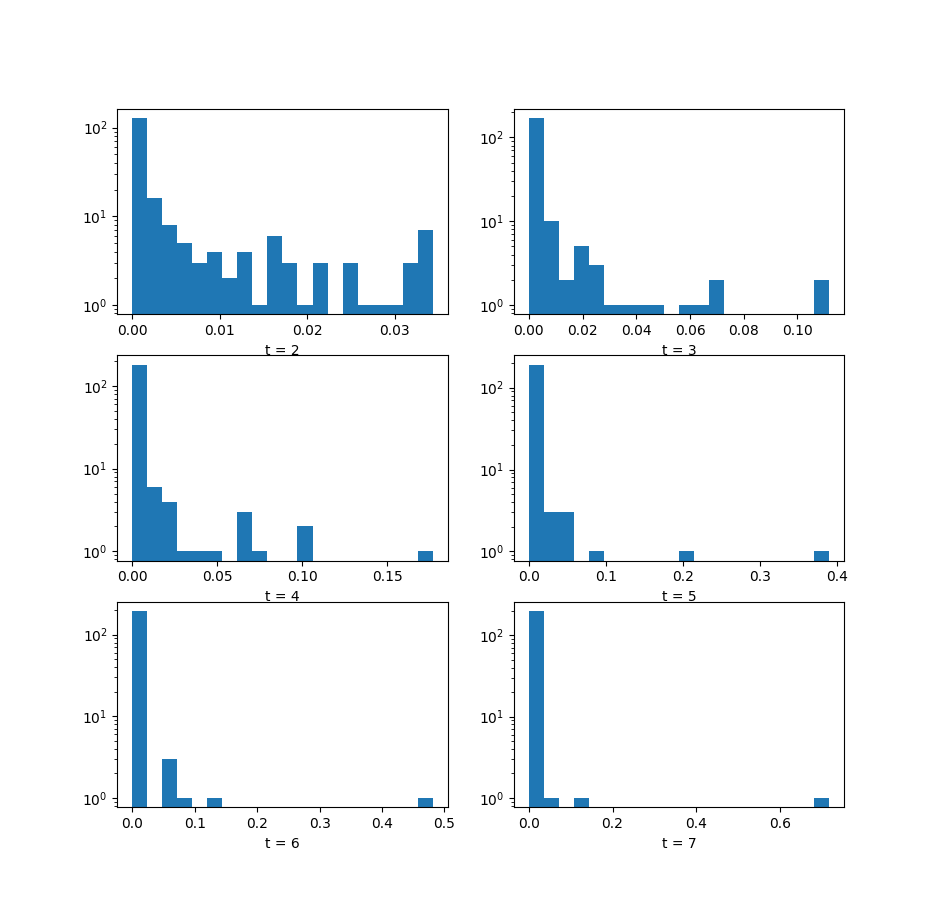
\includegraphics[width=\textwidth]{figures/Figure_weights.png}
  \caption{A histogram of 200 weights after just a few
    iterations. Almost all of the weights are zero at $k = 7$ which
    demonstrates the degeneracy of the particles.}%
  \label{fig:weights}
\end{figure}

%%% Local Variables:
%%% mode: latex
%%% TeX-master: "../main"
%%% End:

\section*{Resampling}
We present two resampling strategies in this section. The overall goal
of all resampling methods is to remove particles with negligible
weights with a high probability and replicate those with high
weights. After resampling, the future particles are more concentrated
in domains of higher posterior probability, which entails improved
estimates. It can, of course, happen that a particle with a low weight
at time $k$ has a high weight at time $k+1$, in which case resampling
could be wasteful. It should also be mentioned that if particles have
(unnormalised) weights with a small variance, resampling might be
unnecessary. This is discussed briefly at the end of this section.

As above, we denote by $\{ x^{(i)}; w^{(i)} \}_{1 \le i \le N}$ the
set of particles with their associated weights at some time $k$ (which
is omitted in the notation). We assume that the weights have already
been normalised such that $\sum_i w^{(i)} = 1$. We further denote by
$\{ \tilde{x}^{(i)}; \tilde{w}^{(i)} \}_{1 \le i \le N}$ the particles
and weights after resampling took place. We require the particles
$\tilde{x}^{(i)}$ to be weighted equally which implies, since we also
require the weights to be normalised that $\tilde{w}^{(i)} = 1/N$.

The use of resampling to improve importance sampling was originally
introduced by Gordon, Salmond and Smith in~\cite{gordon}. The
resampling methods presented here are two of the most popular amongst
the literature, see~\cite{douc}. The most simple resampling strategy,
called \emph{multinomial resampling} is not discussed here due to its
poor performance compared to other techniques. It is mentioned because
it is the method introduced in~\cite{gordon} as part of the\emph{
  bootstrap filter} that uses the prior as the proposal density
(cf.\ Examples~\ref{ex:1} and~\ref{ex:lv1}).

Both methods presented in the following are based on drawing samples
from the point mass distribution
$\sum_{j=1}^N w^{(j)} \delta_{X^{(j)}}$. In practice, this is achieved
by repeated uses of the inversion method, which itself uses the
empirical cumulative distribution function (cdf) associated with the
weights. This is based on the following fact:

\textbf{Claim.}\quad If $U$ is a uniform random variable on $(0,1]$
then $X = F^{-1}(U)$ has distribution $F$, where $F$ is the cdf of $X$
and $F^{-1}(t) = \min \{ x \mid F(x) = t \}$ is the inverse cdf.

\textbf{Proof.}\quad Let $U \sim \mathcal{U} (0,1]$. Then
\begin{align*}
  P(F^{-1}(U) \le x) &= P(\min \{x \mid F(x) = U \} \le x ) && \text{(definition of $F^{-1}$)} \\
                     &= P(U \le F(x)) \\
                     &= F(x) && \text{(definition of distribution of $U$)}\,.
\end{align*}
\hfill$\square$

The inversion method can be explained visually as follows. We plot the
empirical cdf of the weights and sample from
$U \sim \mathcal{U}(0,1]$. We denote the actual value of the sample by
$u$. We then draw a horizontal line from the coordinate $(0,u)$ to the
right until it intersects one of the bars, see
Figure~\ref{fig:ecdf}. The index of the bar that is intersected
determines the new sample.

\begin{figure}
  \centering 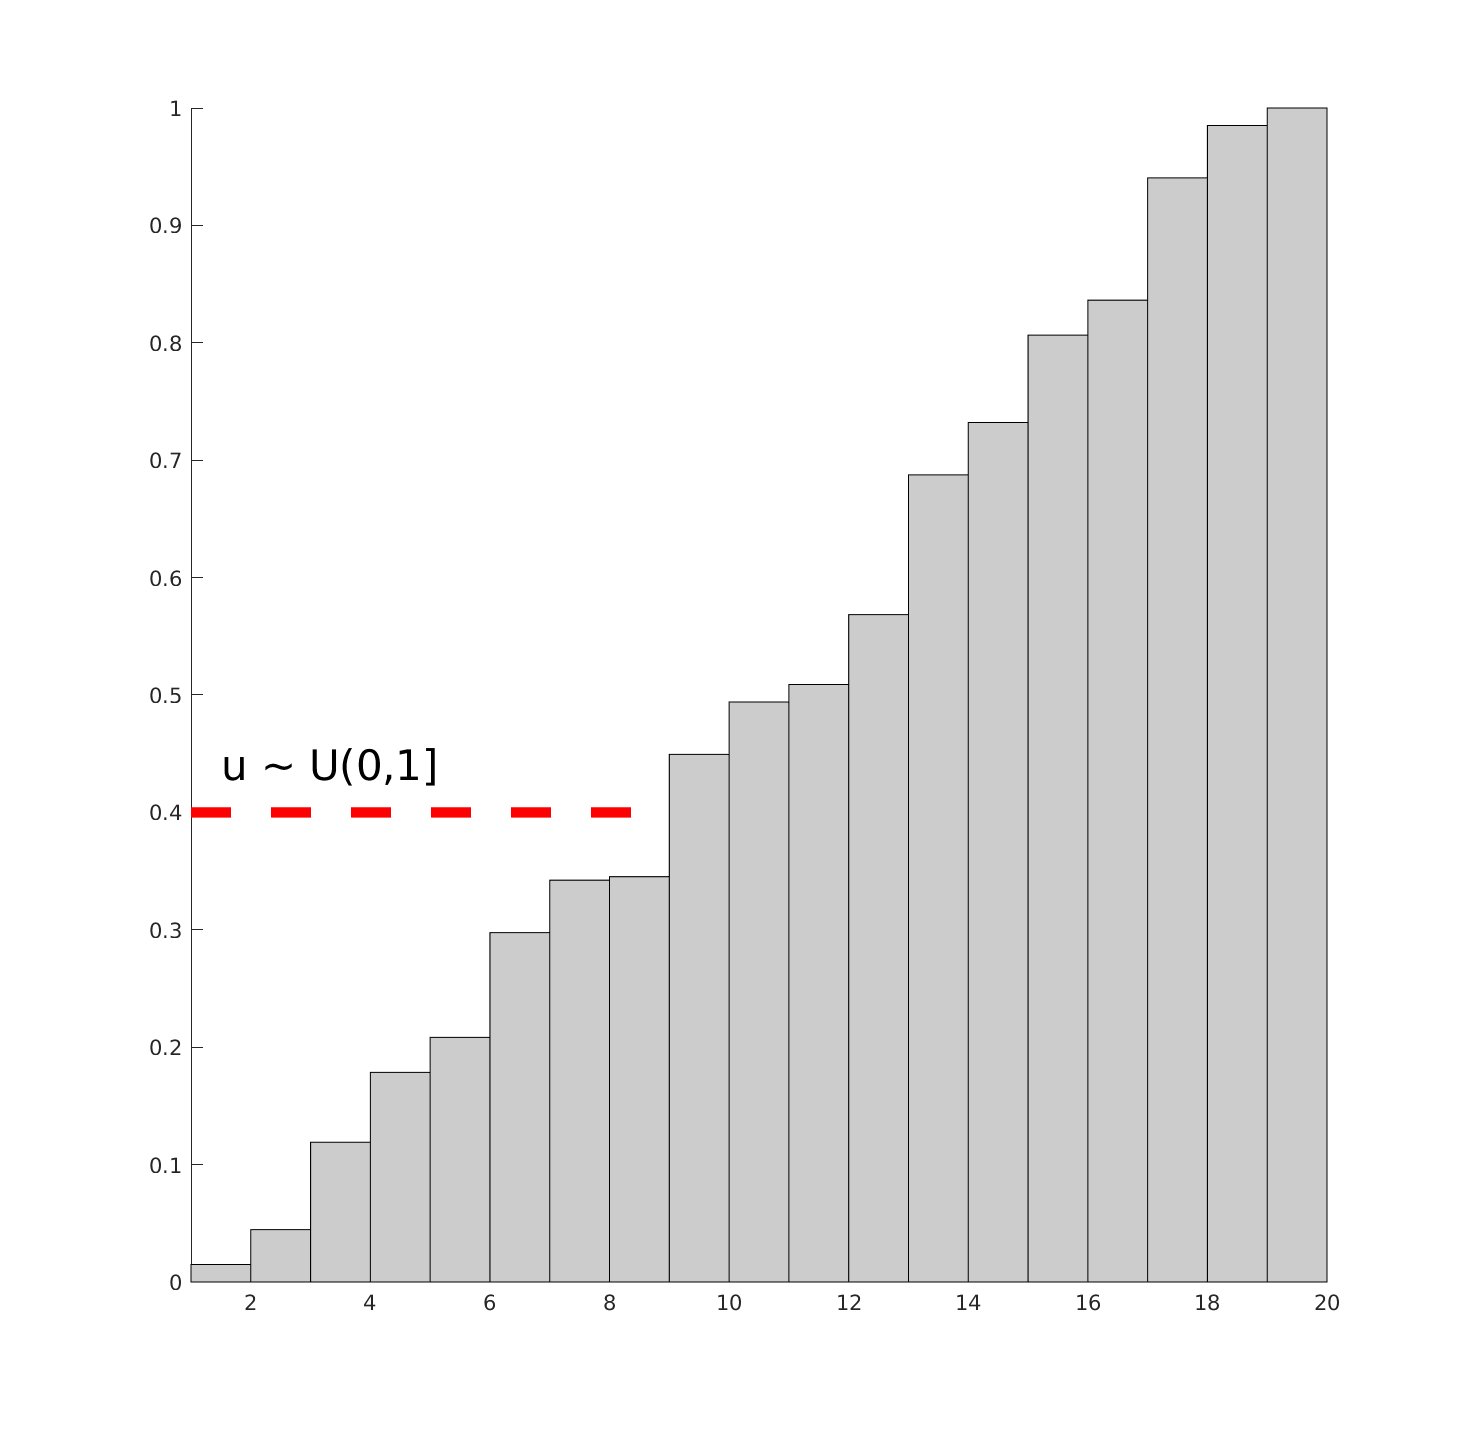
\includegraphics[width=0.5\textwidth]{figures/ecdf.png}
  \caption{Visualisation of the inversion method. The bars represent
    the empirical cumulative distribution function associated with a
    set of 19 weights. The dashed line is horizontally drawn from the
    value of $u$ at the vertical axis until it ``hits'' a bar. The
    index of the bar yields the generated sample (in this case the new
    sample is therefore 9). }
  \label{fig:ecdf}
\end{figure}

In our case, we do not draw just one sample $U$ but we generate $N$
different samples $\{U_i\}_{1 \le i \le N}$ in such a way that they
are sorted in ascending order. For every of these samples (from lowest
to highest) we look for the intersected bar and add its index to a
list. This list then corresponds to the indices of the particles that
should be resampled. Consider the following example: Suppose we had
five particles and the list of indices after the resampling reads
$\{1,3,4,4,5\}$. Then, particles $X^{(1)},X^{(3)},X^{(5)}$ should be
resampled, particle $X^{(4)}$ should even be duplicated. Particle
$X^{(2)}$, however, will be dropped. In other words, the particles
after the resampling are
\begin{gather*}
  \tilde{X}^{(1)}=X^{(1)},\ \tilde{X}^{(2)}=X^{(3)},\ \tilde{X}^{(3)}=X^{(4)},\\
  \tilde{X}^{(4)}=X^{(4)},\ \tilde{X}^{(5)}=X^{(5)}\,.
\end{gather*}

The two strategies presented in the following only differ in the way
the $U_i$s are generated. We summarise the results in
Algorithm~\ref{alg:resampling}.

\begin{algorithm}[htpb]
  \SetAlgoLined
  \KwData{$N$ samples $U_i \sim \mathcal{U}(0, 1]$ sorted in ascending order;\
    list of weights}
  \KwResult{List of indices $I$ that represent that particles to be resampled}
  $C$ = \texttt{cumsum}(weights) \tcp*{Generate the empirical cdf as list of
    accumulated sums\footnotemark}
  $I$ = zeros(N)\;
  $i,j = 0$\;
  \While{$i < N$}{
    \eIf(\tcp*[h]{Found intersecting bar}){
      $U_i < C_j$
    }{
      $I_i = j$\;
      $i = i+1$\;
    } {
      $j = j + 1$\;
    } }
  \caption{Resampling using the empirical cdf}\label{alg:resampling}
\end{algorithm}

\subsection*{Systematic Resampling}
This algorithm separates the sample space into $N$ divisions. One
random offset, drawn from a $\mathcal{U}[0, 1)$ distribution, is used
to choose where to sample from for all divisions. This guarantees that
every sample is exactly $1/N$ apart.

In other words, the $U_i$s are generated by sampling
$\tilde{U} \sim \mathcal{U}[0, 1)$ and defining
\[
  U_i = \frac{\tilde{U} + i-1}{N} \quad \text{for } i = 1, \dotsc, N
  \,.
\]

\subsection*{Stratified Resampling}
\footnotetext{Here, the function \texttt{cumsum} is assumed to work in
  the same way as, for example, MATLAB's or NumPy's \texttt{cumsum}
  function. That is, \texttt{cumsum([1,2,3,4])} should return
  \texttt{[1,3,6,10]}.}  This algorithm is similar to the previous
one, its aim is to make selections relatively uniformly across the
particles. We start by partitioning the $(0,1]$ interval into $N$
disjoint sets,
$(0,1] = (0, 1/N] \cup (1/N, 2/N] \cup \dotsm \cup ((N-1)/N, 1]$. The
$U_i$s are then drawn independently in each of the sub-intervals:
\[
  U_i \sim \mathcal{U}((i-1)/N, i/N]\,.
\]

We mentioned earlier that resampling might be unnecessary if the
weights are sufficiently uniform and we would like to have a criterion
allowing us to check whether resampling should be performed. To that
end the effective sampling size ($ESS$) is often used which can be
estimated using
\begin{equation}
  \label{eq:ESS}
  ESS \approx {\left( \sum_{i=1}^N {\left( w_t^{(i)} \right)}^2
    \right)}^{-1} \,.
\end{equation}
For more details, see~\cite[179]{arulampalam}. If the variance of the
weights is maximal, \ie, if all but one of the weights are zero, the
value of $ESS$ is 1. If, however, the weights all have the same value
$w_t^{(i)} = 1/N$ the value of $ESS$ is $N$, since
\[
  {\left( \sum_{i=1}^N {\left( \frac{1}{N} \right)}^2 \right)}^{-1} =
  {\left( N \frac{1}{N^2} \right)}^{-1} = N \,.
\]
Therefore, we will only resample if $ESS$ is below a certain
threshold, e.\,g.\ $N/2$.

We have now gathered everything we need to implement a particle
filter, since essentially particle filters are simply a combination of
sequential importance sampling and one of the resampling strategies
(or, of course, any other resampling algorithm not presented
here). Consequently, these methods are sometimes called
\emph{Sequential Importance Sampling with Resampling} abbreviated by
SIR or SIS/R. Other popular names include \emph{Bootstrap filter},
\emph{Monte Carlo filter}, \emph{Survival of the fittest} or
\emph{Condensation algorithm}.

%%% Local Variables:
%%% mode: latex
%%% TeX-master: "../main"
%%% End:

\section*{Implementation}
In this section we present an implementation of a particle filter in
C++. The particle filter itself is implemented as a
dependency-free\footnote{The library can be configured to run some
  parts in parallel. In that case the program has to be linked against
  Intel's Threading Building Blocks (TBB) library~\cite{intel}. If the
  parallel capabilities are not used, the library depends only on the
  C++ standard library.} header-only generic library that, while being
easy to set up and use, is versatile and can be used with a wide
variety of problems. This is demonstrated by three examples, two of
which are based on the same problem but are using different prior and
proposal distributions.

The code can be found at
\url{github.com/nilsfriess/ParticleFilter}. The GitHub repository
contains a CMake~\cite{cmake} project containing the actual library in
the folder \texttt{libs/smcpf} and three examples located in the
folder \texttt{apps}. Information about the dependencies of the
individual examples and instructions on how to build and run them can
be found in the \texttt{README.md} file inside the root folder of the
repository. The \texttt{data} folder contains sample data to use with
the examples and scripts that were used to generate the sample data.

The library consists of the following classes (and their respective
header files)
\begin{itemize}
\item Particle \texttt{(particle.hh)}
\item ParticleFilter \texttt{(particlefilter.hh)}
\item Model \texttt{(model.hh)}
\item History \texttt{(history.hh)}
\end{itemize}
All of these classes lie in a namespace \texttt{smcpf} and are
templated to allow for arbitrary particle types, e.\,g.\ the
\texttt{Particle} class, that holds the value and weight of a single
particle is of the following form
\begin{minted}{cpp}
template <class PT> 
class Particle {
private:
  PT m_value;
  double m_weight;
...
}; 
\end{minted}
where the particle type \texttt{PT} could take values of some finite
set, be a real number (\ie, a \texttt{double}) or a $n$-dimensional
vector etc. The \texttt{ParticleFilter} class implements the
algorithms introduced above. It takes the following template
parameters
\begin{minted}{cpp}
template <class PT, class OT, 
          size_t N,  
          typename... Args>
class ParticleFilter { ... }

\end{minted}
where \texttt{PT} and \texttt{OT} denote the type of particle and
observation, respectively and \texttt{N} is the number of
particles. The last template parameter \texttt{Args} is
\emph{parameter pack} that can hold an arbitrary number of additional
arguments of any type. The use for such arguments is explained in the
description of the \texttt{Model} class below.

The library can be configure to run parts of it in parallel, \eg the
particle evolution (see below). To enable this feature, one has to
define the prepocessor constant \texttt{PF\_USE\_PARALLEL} before the
header file \texttt{particlefilter.hh} is included, \eg by
\begin{minted}{cpp}
#define PF_USE_PARALLEL
#include <particlefilter.hh>
\end{minted}

Internally, this uses the C++17 \texttt{execution} header from the C++
standard library that depends on Intel's TBB
library~\cite{intel}. This means, if \texttt{PF\_USE\_PARALLEL} is
set, the TBB header files have to be available for the compiler and
the program has to be linked against the library \texttt{tbb}. Not
using the parallel capabilities of the library does neither change the
way it has to be used nor does it limit its capabilities. It only
affects how the internal algorithms are run.

Apart from these compile-time parameters, to construct a
\texttt{ParticleFilter} one also needs to provide an instance of a
\texttt{Model}, a resampling strategy\footnote{At the moment, only
  systematic resampling is implemented.}, a resampling threshold and
an initial seed for the random number generator (rng). Additionally, a
boolean parameter that specifies whether some information from every
time step should be held in memory has to be given (\eg for debugging
or plotting, see examples below). Only the first parameter is
mandatory, i.\,e.\ the signature of the constructor of the
\texttt{ParticleFilter} class is given by
\begin{minted}{cpp}
ParticleFilter(
    Model<PT, OT, Args...> *t_model,
    bool t_enable_history = false,
    ResamplingStrategy t_strategy = ResamplingStrategy::RESAMPLING_SYSTEMATIC,
    double t_threshold = 0.5, 
    double t_seed = 0)
\end{minted}
The value of \texttt{t\_strategy} can either be the default
\texttt{RESAMPLING\_SYSTEMATIC} or \texttt{RESAMPLING\_NONE}, both of
which are defined in the enumeration \texttt{ResamplingStrategy}. The
value of \texttt{t\_threshold} is used to decide when to actually
perform resampling. At each time step an estimate of the effective
sampling size is computed using~\eqref{eq:ESS}. The particles are only
resampled if this value is below \texttt{t\_threshold} $\times$
\texttt{N}. Thus, \texttt{t\_threshold} should take values between
zero and one (since ESS takes values between 1 and \texttt{N}), where
a value of zero implies that the particles are never resampled and one
leads to resampling being performed at each step. Before explaining
the methods defined inside the \texttt{ParticleFilter} we discuss the
\texttt{Model} class.

This class is implemented as an abstract base class (sometimes called
\emph{interface}), meaning that the class itself cannot be
instantiated. Therefore, in order to define a model, a class that is
derived from \texttt{Model} has to be implemented. The class is also
templated with the following parameters
\begin{minted}{cpp}
template <class PT, 
          class OT, 
          typename... Args> 
class Model { ... }
\end{minted}
where \texttt{PT} and \texttt{OT} are again the particle and
observation type. To explain the usage of the parameter pack
\texttt{Args} we first discuss the virtual functions of the class:
\begin{minted}{cpp}
virtual PT zero_particle() = 0;

virtual void sample_prior(Particle<PT> &t_particle) = 0;

virtual double update_weight(const Particle<PT> &t_particle_before_sampling,
                             const Particle<PT> &t_particle_after_sampling,
                             const OT &t_observation, 
                             Args... t_args) = 0;

virtual PT sample_proposal(const Particle<PT> &t_particle,
                           const OT &t_observation, 
                           Args... t_args) = 0;
\end{minted}
All these methods are \emph{pure virtual} methods meaning that a model
class that derives from this class must implement all four of
them. They all get automatically called by the
\texttt{ParticleFilter}. The first method should return a value of
type \texttt{PT} that represents zero, \ie, in the one dimensional
case where \texttt{PT = double} this should be 0, if \texttt{PT} is
\eg two dimensional, this method should return the 2D zero vector and
analogously for higher dimensions and other particle types. The method
\texttt{sample\_prior} is used to initialise the set of particles. It
has to set the value of the given particle \texttt{t\_particle} using
the \texttt{set\_value} method of the particle. This is different from
the \texttt{update\_weight} and \texttt{sample\_proposal} methods that
\emph{do not} alter the particle themselves. Rather they should return
the value the the particle's weight should get multiplied by and the
particle's new value, respectively (see examples below).

The first parameter of the \texttt{update\_weight} method is the
particle before \texttt{sample\_proposal} is called and the second
after it is called. This is useful, since the developer cannot specify
the order in which these two methods are called. However, some models
require the value of the particle before it has been updated (cf.\
Example~\ref{ex:lv1}) and some after the sampling step (cf.\
Example~\ref{ex:1} and~\ref{ex:lv2}). The type of the last parameter
\texttt{t\_args} of both methods is specified by the template
parameter pack \texttt{Args}. It can be used to supply an arbitrary
number of additional parameters of arbitrary types to these methods.
This can be used if the proposal pdf and weight update function depend
on additional parameters like the current time step, which is the case
in all of the following examples. The types provided as \texttt{Args}
to the \texttt{Model} class and those provided to the
\texttt{ParticleFilter} must match, otherwise the program will not
compile. The following simple example is used to demonstrate how a
model can be defined.

\begin{example}\label{ex:1}
  This example has been studied in a number of publications before,
  see for example~\cite{arulampalam,gordon,kitagawa}. The
  implementation can be found in the file
  \texttt{apps/example1/main.cc}. Let
  \begin{align*}
    p(x_0) &= \mathcal{N}(0,0.5)\\
    p(x_n \mid x_{n-1}) &= \mathcal{N}(x_n;\, h_n(x_{n-1};n), \sigma_{\text{sys}})\\
    p(y_n \mid x_n) &= \mathcal{N}(y_n;\, \frac{{x_n}^2}{20},
                      \sigma_{\text{obs}})
  \end{align*}
  where
  \begin{equation}
    \label{eq:ex1:h}
    h_n(x_{n-1};n) = \frac{1}{2}x_{n-1} + \frac{25 x_{n-1}}{1 + x_{n-1}^2} + 8 \cos(1.2n) \\
  \end{equation}
  and $\mathcal{N}(\mu, \sigma)$ denotes a Gaussian distribution with
  mean $\mu$ and variance $\sigma$ and $\mathcal{N}(x; \mu, \sigma)$
  denotes a Gaussian pdf with mean $\mu$ and variance $\sigma$
  evaluated at $x$. We choose $\sigma_{\text{sys}} = 10$ and
  $\sigma_{\text{obs}} = 1$.

  Since both the particles and observations are one-dimensional we set
  \texttt{PT = double,\ OT = double}. Note that $h$ defined
  in~\eqref{eq:ex1:h} depends on the index of the current time step
  $n$. Therefore, we provide one additional template parameter, \ie,
  we set \texttt{Args = int}. Hence, the model could be defined as
\begin{minted}{cpp}
class ExampleModel : public Model<double, double, int> {
\end{minted}
  Here, the zero particle is simple the value \texttt{0.0} and the
  prior is a Gaussian, centred at 0 with variance 0.5.
\begin{minted}{cpp}
...
public:
  virtual double zero_particle() override { return 0.0; }

  virtual void sample_prior(Particle<double> &t_particle) override {
    t_particle.set_value(m_prior(m_gen));
  }
\end{minted}
  where \texttt{m\_gen} and \texttt{m\_prior} are defined as
\begin{minted}{cpp}
...
private:
  std::mt19937 m_gen;
  std::normal_distribution<> m_prior{0, 0.5};
\end{minted}
  The class \texttt{std::mt19937} defines a pseudo rng based on the
  \emph{Mersenne Twister} algorithm.

  To implement the remaining two methods we first have to choose a
  proposal density. For simplicity, we use the prior
  $p(x_n \mid x_{n-1})$, \ie, we implement a bootstrap particle
  filter.  The recursive weight update
  formula~\eqref{eq:weight_update} then simplifies to
  \[
    w_k^{(i)} \propto w^{(i)}_{k-1} p(y_k \mid x_k^{(i)}) \,,
  \]
  and we obtain
\begin{minted}{cpp}
  virtual double
  update_weight(const Particle<double> & /*t_particle_before_sampling*/,
                const Particle<double> &t_particle_after_sampling,
                const double &t_observation, int /*t_step*/) override {
    auto pval = t_particle_after_sampling.get_value();
    auto mean = (pval * pval) / 20.0;
    auto var = 1.0;

    return normal_pdf(t_observation, mean, var);
  }
\end{minted}
  The function \texttt{normal\_pdf(double, double, double)} is defined
  in the file \texttt{helper.hh} and simply implements a Gaussian pdf.
  Note that the \texttt{update\_weight} method does not return the new
  value of the weight but rather the value the weight should be
  multiplied with, \ie, in our case $p(y_k \mid x_k^{(i)})$.

  Since in this case the proposal is the prior, the
  \texttt{sample\_proposal} method is a straightforward implementation
  of $p(x_k^{(i)} \mid x_{k-1}^{(i)})$ defined by the model above.
\begin{minted}{cpp}
  virtual double sample_proposal(const Particle<double> &t_particle,
                                 const double & /*t_observation*/,
                                 int t_step) override {
    auto pval = t_particle.get_value();
    auto mean = pval / 2.0 + (25 * pval) / (1 + pval * pval) +
                8 * std::cos(1.2 * (t_step));
    auto var = 10.0;

    std::normal_distribution<> proposal{mean, var};
    return proposal(m_gen);
  }
\end{minted}
  With these four methods the model is fully defined and can be used
  to construct a \texttt{ParticleFilter}. In the file
  \texttt{apps/example1/main.cc} two additional methods
  \begin{itemize}
  \item \mint{cpp}|void load_observations(const std::string
    &t_filename)|
  \item \mint{cpp}|std::optional<std::pair<double, double>>
    next_observation()|
  \end{itemize}
  are defined. The first method loads observations from a \texttt{csv}
  file (comma-separated values) and the second method returns a new
  observation each time it is called until all observations have been
  read. An observation consists of a time index and the actual
  observation. The artificial observations can be generated using the
  Python script \texttt{data/example1/gen\_obs\_ex1.py} that generates
  100 random samples $x_k \sim p(x_k \mid x_{k-1})$ where
  $x_0 \sim p(x_0)$. The observations are then generated by squaring
  these values, dividing them by 20 and perturbing them by additive
  Gaussian noise such that they are distributed according to
  $p(y_k \mid x_k)$. These artificial observations and the
  corresponding time steps are then written to a file that can be read
  by the method \texttt{load\_observations}.

  With this model we con now easily implement the actual particle
  filter:
\begin{minted}{cpp}
int main() {
  constexpr size_t N = 400;

  typedef smcpf::ParticleFilter <double, // Type of particle
                                 double, // Type of observation
                                 N,      // Number of particles
                                 int>    // index of observation
                                 PF;
  ExampleModel model;

  PF pf(&model, true);
  ...
\end{minted}
  The observations are automatically loaded inside the constructor of
  the model and the initial set of particles is initialised inside the
  constructor of the \texttt{ParticleFilter}. To run the actual
  filtering we have to call the method \texttt{evolve}, defined as
\begin{minted}{cpp}
void ParticleFilter::evolve(OT t_observation,  Args... t_args)
\end{minted}
  This method calls the \texttt{sample\_proposal} and
  \texttt{update\_weight} method of the model for each of the
  particles. If the template parameter \texttt{parallel} is set to
  true, this is done in parallel. This requires no extra care since
  the particles are all independent and altering the value or weight
  of one particles does not affect any of the other particles.  In
  addition, this method checks whether resampling is necessary and
  possibly resamples the particles. Resampling, however, cannot be
  easily parallelized (there are some publications discussing the
  parallelization of resampling algorithms, see \eg~\cite{murray}).

  The \texttt{evolve} method has to be called at each time step. Using
  the \texttt{next\_observation} method of our model we do this as
  follows
\begin{minted}{cpp}
  while (auto obs = model.next_observation()) {
    pf.evolve(obs.value().second, obs.value().first);
  }
\end{minted}
  Using the method
\begin{minted}{cpp}
PT ParticleFilter::weighted_mean()
\end{minted}
  one can obtain a Monte Carlo estimate of the expectation of a random
  variable with pdf $p(x_k \mid y_{1:k})$ at each time step $k$. Since
  we set the \texttt{history} flag to \texttt{true}, these means are
  all held in memory and we can read them after all observations have
  been processed. To that end, the \texttt{ParticleFilter} class
  provides a method
\begin{minted}{cpp}
  template <class PTWriter, class ArgWriter>
  void write_history(std::ostream &t_out, 
                     PTWriter t_writer,
                     ArgWriter t_awriter, 
                     char t_separator = ',')
\end{minted}
  that writes the contents of the history to the output stream
  \texttt{t\_out} (\eg a file stream) using the functors
  \texttt{PTWriter} and \texttt{ArgWriter}, which have to be
  implemented such that they convert values of types \texttt{PT} and
  \texttt{Args...} to \texttt{std::strings} (\ie, they define how to
  print these values). For a detailed description on the usage of this
  method see the example files and the comments in the definition of
  the particle filter class.

  Figure~\ref{fig:ex1} shows the plot of one exemplar run together
  with the generated observations and simulated values using the model
  and particle filter described above.
  
\end{example}
The following two examples are based on the same problem and
demonstrate how third-party libraries can be used to define arbitrary
particle types.

\begin{example}[Lotka Volterra using bootstrap filter]\label{ex:lv1}
  Given approximations of the population size of a certain species
  (the \emph{predators}) we want to estimate the quantity of another
  species (the \emph{preys}) and estimate their respective population
  sizes. The predators and preys are assumed to follow the so called
  \emph{Lotka-Volterra model}. This model is mainly described by the
  following system of differential equations:
  \begin{equation}
    \label{eq:lotka}
    \begin{aligned}
      \frac{\dx}{\dt} &= \alpha x - \beta xy \,, \\
      \frac{\dy}{\dt} &= \delta xy - \gamma y \,,
    \end{aligned}
  \end{equation}
  where
  \begin{itemize}
  \item $x$ is the number of prey;
  \item $y$ is the number of predator;
  \item $\alpha, \beta, \gamma, \delta$ describe the interaction of
    the predator and prey.
  \end{itemize}
  We assume that we can observe the predators (i.e.\ $y$) but not the
  number of prey. To this end, we will create artificial values for
  the predators and preys by solving the Lotka Volterra equations with
  some initial values. We then ``observe'' the number of predator by
  perturbing the exact computed values at discrete points in time by
  additive Gaussian noise. These observations are then used as inputs
  for the particle filter.

  Formally, this model is defined by the following equations
  \begin{equation}
    \label{eq:lv}
    \begin{aligned}
      p(\bm{x}_0) &= \mathcal{N}(\bm{\mu}_0, \bm{I})\,, \\
      p(\bm{x}_t \mid \bm{x}_{t-1}) &= \mathcal{N}(\bm{x}_t;\, M(\bm{x}_{t-1}; t), \bm{I})\,, \\
      p(y_t \mid \bm{x}_t) &= \mathcal{N}(y_t;\, F(\bm{x}_{t}), 2) \,,
    \end{aligned}
  \end{equation}
  where $\bm{\mu}_0 = {(4, 6)}^T$, $\bm{I}$ denotes the $2 \times 2$
  identity matrix, $M(x_{t-1}; t)$ is the solution of the Lotka
  Volterra equations from time $t-1$ to $t$ with initial value
  $x_{t-1}$ and $F(\bm{x})$ extracts the value of the predator from
  the vector $\bm{x} = {(x_1, x_2)}^T \in \R^2$, \ie,
  \begin{equation}
    \label{eq:lv1:obs}
    F(\bm{x}) = F({(x_1, x_2)}^T) = x_2
  \end{equation}
  or equivalently
  \begin{equation}
    \label{eq:lv1:obs2}
    F(\bm{x}) = \bm{H} \bm{x}\,,
  \end{equation}
  where $\bm{H} = (0, 1) \in \R^{1 \times 2}$ is an \emph{observation
    matrix}. Additionally, we assume the values of
  $\alpha, \beta, \gamma, \delta$ are known to be
  \[
    \alpha = \gamma = 1 \qquad \text{and} \qquad \beta = \delta =
    0.1\,.
  \]

  To define a model class, we proceed as in the previous
  example. Since the particles take values in $\R^2$ we cannot use
  \texttt{double} values. Since this example should also demonstrate
  how third-party libraries can be used, instead of using
  \texttt{std::vector} or \texttt{std::array} to model the 2D vectors
  we use a vector class from the linear algebra library
  \emph{Armadillo}~\cite{armadillo}. The model can then be defined as
\begin{minted}{cpp}
class LotkaVolterra : public smcpf::Model<arma::dvec, double, double> {
\end{minted}
  where the first parameter \texttt{arma::dvec} defines the particle
  type (\ie, the two dimensional vector holding the value of the prey
  and predator, respectively), the second parameter is again the
  observation type and the additional \texttt{double} parameter
  denotes the type of the time steps.

  As above, we need to override the four pure virtual methods of the
  \texttt{Model} class. Here, a zero particle is the zero vector, \ie,
\begin{minted}{cpp}
  arma::dvec zero_particle() override { return {0, 0}; }
\end{minted}
  To sample from the prior we use the functor
  \texttt{BivariateGaussian} that can be found in the
  \texttt{functors.hh} file in the \texttt{apps/example2} folder. This
  functor represents a two-dimensional Gaussian
  distribution. Internally it uses a library called
  \emph{StatsLib}~\cite{stats} which provides a wide variety of
  statistical distributions and helper functions, in particular it
  provides classes and methods to sample from and evaluate
  multivariate normal distributions. After setting up the prior in the
  constructor of the \texttt{LotkaVolterra} class
\begin{minted}{cpp}
    const arma::dvec mu{{4}, {6}};
    const arma::dmat sigma{{1, 0}, {0, 1}};
    m_prior = BivariateNormal(mu, sigma);
\end{minted}
  we can use it to define the \texttt{sample\_prior} method
\begin{minted}{cpp}
  virtual void sample_prior(smcpf::Particle<arma::dvec> &t_particle) override {
    t_particle.set_value(m_prior());
  };
\end{minted}
  As in the previous example, to define the remaining two methods we
  have to choose a proposal density. In this example, we again
  implement a bootstrap filter, \ie, we use
  $p(\bm{x}_t \mid \bm{x}_{t-1})$ as the proposal and obtain
\begin{minted}{cpp}
  virtual double update_weight(
      const smcpf::Particle<arma::dvec> & /*t_particle_before_sampling*/,
      const smcpf::Particle<arma::dvec> &t_particle_after_sampling,
      const double &t_observation, double /*t_time*/) override {
    return stats::dnorm(t_observation,
                        extract_predator(t_particle_after_sampling), 2);
  }

  arma::dvec sample_proposal(const smcpf::Particle<arma::dvec> &t_curr_particle,
                             const double & /* t_observation */,
                             double t_time) override {
    const auto mu = evolve(t_curr_particle, t_time);
    const arma::dmat cov = {{1, 0}, {0, 1}};

    return BivariateNormal(mu, cov)();
  }
\end{minted}
  The method \texttt{stats::dnorm} from the \emph{StatsLib}
  library~\cite{stats} used in the \texttt{weight\_update} method
  provides the density function of a one-dimensional Gaussian. The
  method \texttt{extract\_predator} implements the observation
  function $F(\bm{x})$ given in~\eqref{eq:lv1:obs}.

  Inside the \texttt{sample\_proposal} method the particle is evolved
  using the model's method \texttt{evolve} that simply solves the
  Lotka Volterra equations at the current time step using the
  \texttt{odeint} methods from the C++ library Boost~\cite{boost}.

  The remaining methods of the class are again helper functions to
  process the previously generated observations. Setting up and
  running the particle filter is then done similarly as in the first
  example. Figure~\ref{fig:ex2} shows the exact values of the
  predators and preys, respectively, and the observations that were
  given to the particle filter. The two dotted lines show the sample
  means of the filtered posterior, \ie, the simulated values for the
  predators and preys.

\end{example}

The previous two examples both implement a bootstrap filter. The next
example is based on the same model as Example~\ref{ex:lv1} but uses a
different proposal.

\begin{example}[Lotka Volterra using optimal proposal]\label{ex:lv2}
  Consider the model from the previous example defined
  in~\eqref{eq:lv}. In~\cite{Doucet2000} Doucet, Godsill and Andrieu
  showed that for models of this form an optimal proposal density
  exists in the sense that the variance of the importance weights is
  minimised.

  In general, this proposal is given by
  \begin{align*}
    q(x_k \mid x^{(i)}_{k-1}, y_k) &= p(x_k \mid x_k^{(i)}, z_k)
  \end{align*}
  Substituting this into~\eqref{eq:weight_update} yields
  \[
    w_k^{(i)} \propto w_{k-1}^{(i)} p(y_k \mid x_{k-1}^{(i)}).
  \]
  As is illustrated in~\cite[Example 3]{Doucet2000} for models with
  nonlinear internal dynamics and linear measurements both
  $p(x_k \mid x_k^{(i)}, z_k)$ and $p(y_k \mid x_{k-1}^{(i)})$ are
  Gaussian. Our model obviously fulfils these requirements and we can
  define $p(x_k \mid x_k^{(i)}, z_k)$ and $p(y_k \mid x_{k-1}^{(i)})$
  as follows (see~\cite{Doucet2000} for the derivation). First let
  \begin{align*}
    \bm{\Sigma}_t &= {\left(\bm{I} + \frac{1}{2} \bm{H}^T \bm{H}\right)}^{-1}\,\\
    \bm{\mu}_t &= \bm{\Sigma}_t \left(M(\bm{x}_{t-1}; t) + \frac{1}{2} H^T y_t\right)\,.
  \end{align*}
  Then
  \begin{equation}
    \label{eq:optimal_proposal}
    p(\bm{x}_t \mid \bm{x}_{t-1}, y_t) = \mathcal{N}(\bm{x}_t;\, \bm{\mu}_t, \bm{\Sigma}_t)
  \end{equation}
  and
  \begin{equation}
    \label{eq:optimal_weight}
    p(y_t \mid \bm{x}_{t-1}) = \mathcal{N}(y_t; \, \bm{H} M(\bm{x}_{t-1}; t), \,  \bm{H} \bm{H}^T + 2)\,.
  \end{equation}
  Since this choice of proposal density minimises the variance of the
  weights which implies an increase of the effective sampling size
  compared to the previous approach, we expect resampling to be
  performed less often. This can be easily checked using the output
  files that the examples generate, since the history also saves
  whether resampling has been performed at a particular time step. And
  indeed, while the previous example requires resampling to be
  performed at around 20 steps (of a total of 50 steps), using the
  optimal proposal this number is reduced to five resampling steps
  (both exemplar runs used 5000 particles and a resampling threshold
  of 50\%). This also has an effect on the speed of the particle
  filter since resampling is the only step that is not easily
  parallelized. Therefore, one wants to resample as few times as
  possible.

  The code for this example can be found in the folder
  \texttt{apps/example3} but is essentially the same as in the
  previous example with the \texttt{update\_weight} and
  \texttt{sample\_proposal} methods altered to
  implement~\eqref{eq:optimal_weight} and~\eqref{eq:optimal_proposal}.
  For completeness, the results using this example are plotted in
  Figure~\ref{fig:ex3}.
\end{example}

\begin{landscape}
  \begin{figure}
    \centering
    \includegraphics[width=\linewidth,height=\textheight,keepaspectratio]{figures/figure_ex1.pdf}
    \caption{Results from one exemplar run using the model and
      particle filter described in Example~\ref{ex:1}. The black line
      with crosses shows the exact values, the dotted line shows the
      generated observations and the red line (the line without
      points) is the result using 400 particles, systematic resampling
      and a resampling threshold of 50\%.}%
    \label{fig:ex1}
  \end{figure}
\end{landscape}

\begin{landscape}
  \begin{figure}
    \centering
    \includegraphics[width=\linewidth,height=\textheight,keepaspectratio]{figures/figure_ex2.pdf}
    \caption{Results from one exemplar run using the model and
      particle filter described in Example~\ref{ex:lv1}. Here, 1000
      particles and the default values of the particle filter were
      used.}%
    \label{fig:ex2}
  \end{figure}
\end{landscape}

\begin{landscape}
  \begin{figure}
    \centering
    \includegraphics[width=\linewidth,height=\textheight,keepaspectratio]{figures/figure_ex3.pdf}
    \caption{Results from one exemplar run using the model and
      particle filter described in Example~\ref{ex:lv2}. Here, 1000
      particles and the default values of the particle filter were
      used.}%
    \label{fig:ex3}
  \end{figure}
\end{landscape}


%%%Local Variables:
%%% TeX-command-extra-options: "-shell-escape"
%%% mode: latex
%%% TeX-master: "../main"
%%% End:
 
















































 
\printbibliography

\end{document}

 
%%% Local Variables:
%%% mode: latex
%%% TeX-master: t
%%% TeX-command-extra-options: "-shell-escape"
%%% End:
